

\documentclass[conf]{new-aiaa}
%\documentclass[journal]{new-aiaa} for journal papers
\usepackage[utf8]{inputenc}

\usepackage{graphicx}
\usepackage{amsmath}
\usepackage[version=4]{mhchem}
\usepackage{siunitx}
\usepackage{longtable,tabularx}
\usepackage{listings}
\usepackage{float}
\setlength\LTleft{0pt} 

\title{First Draft: Circumnavigation and obstacle avoidance guidance for UAV monitoring a ground target using Vector Fields}

\author{Jay P. Wilhelm\footnote{Assistant Professor, Department of Mechanical Engineering, 251 Stocker Center, AIAA Senior Member.} and Second B. Author Jr.\footnote{Insert Job Title, Department Name, Address/Mail Stop, and AIAA Member Grade (if any) for second author.}}
\affil{Ohio University, Athens, OH, 45701}

\begin{document}

\maketitle

\begin{abstract}
Circumnavigation of a moving ground target using a UAV requires guidance to maintain a standoff distance. Fixed wing aircraft are unable to directly follow over a ground target and must turn to maintain flight. Vector Field (VF) guidance was investigated as a circumnavigation method that would converge, circulate, and track a moving target using a constant radius circle with the target as a center. Parameters of the VF were explored to understand performance and capabilities of the field. In addition, obstacles may be present and can be represented by a VF that pushes away to achieve avoidance. The VF guidance circumnavigation and obstacle avoidance was simulated using a UAV Dubins vehicle that followed a target with an unknown path.
\end{abstract}

\section{Nomenclature - SECTION NEEDS TO BE COMPLETED OR OMITTED}

{\renewcommand\arraystretch{1.0}
\noindent\begin{longtable*}{@{}l @{\quad=\quad} l@{}}
$A$  & amplitude of oscillation \\

\end{longtable*}}

\section{Introduction}
\lettrine{C}{ircumnavigation} of a moving target using an aerial vehicle requires a guidance system to control the surveillance aircraft's heading. There are several methods to guide a vehicle to maintain a radius around a target, but the two most prominent are direct guidance laws and Vector Fields (VF). Further complication of guidance requirements comes from a moving target where the path is not known. Typically, the target and vehicle position, and velocity are necessary for the guidance system. Additional features of a guidance system may include obstacle or areas of avoidance. The VF guidance generation was investigated to determine tracking performance of an aerial vehicle to circumnavigate (circle) a target that is moving and avoid designated areas.

\section{Literature Review}
Guidance for a UAV that is moving faster than another target, assumed in this case to be a ground vehicle, may be achieved using several different methods. Three recurring types of guidance seen for UAVs include Potential Fields, classical optimal laws, and Vector Fields (VF). Various methods are used to generate Potential Fields, where obstacles are characterized by areas of high potential and the area of lowest potential contains the goal or end point {\cite{goerzen2010survey}}. The UAV is guided from an initial position in the field, following a path of descending potential, until it reaches the area of lowest potential {\cite{goerzen2010survey}}. While potential field methods may be utilized for some guidance scenarios, they have inherent limitations {\cite{koren1991potential}} and are not a feasible method for circumnavigation of a target. Classical control laws were developed {\cite{oliveira2016moving,kaminer1998trajectory}}, are typically non-linear, and require direct control over a vehicle's heading. Vector Field methods and control laws found in literature assume constant UAV velocity {\cite{chen2009tracking}}, which is controlled using a separate system. Classical control laws were found to be complicated in terms of required calculations, and are unsuitable in this case due to their inability to circumnavigate a target. VF methods were investigated further due to their ability to provide circumnavigation of a moving and non-moving target. The VFs come in several different forms where the initial and final concept of generating the field are fundamentally different. The two primary methods considered in the generation of VFs for guidance are Lyapunov {\cite{frew_tracking_2012}} and Gon\c{c}alves {\cite{goncalves_circulation_2010}} or Gradient Vector Fields (GVF), which generate fields using completely different fundamental mechanisms. Lyapunov and GVF both appear to generate similar VFs for basic shapes (ex, circle), and are undefined at the origin (x=0,y=0). The GVF has additional features that allow for time-varying scenarios, where the surfaces move with respect to time, and the ability to support more advanced surfaces than Lyapunov.

\section{The Lyapunov Vector Field}
Lyapunov VFs can be generated given a Lyapunov function as defined in Frew {\cite{frew_tracking_2012}}. The exact method of transforming a Lyapunov function into a VF equation can be found {\cite{rosier1992homogeneous,chen2013uav,chen2009tracking}}. Circular VF guidance, or circumnavigation, using a Lyapunov equation can be achieved from Equation \ref{eq:lyapunovvf} where $v$ is the desired UAV velocity, $r$ is the UAV distance from the center of the field, $r_d$ is the desired circle radius, and $x$ and $y$ are the UAV positions. The Lyapunov VF can be built from a variety of continuous shapes and may include a constant wind field by summing an additional vector.

\begin{equation}\label{eq:lyapunovvf}
\overrightarrow{V}_{Lyapunov} = \frac{v}{r^2+r_d^2} \begin{bmatrix} -x (r^2-r_d^2) - y (2 r r_d^2) \\ -y (r^2-r_d^2) - x (2 r r_d^2)\end{bmatrix}
\end{equation}

\section{The Gon\c{c}alves Vector Field}
The GVF is fundamentally an interaction of two surfaces that produces a convergence and circulation path where the surfaces intersect {\cite{goncalves_circulation_2010,goncalves_artificial_2009,goncalves_vector_2010,goncalves_coordination_2013}}. The functions to express the surfaces ($\alpha_i:\mathbb{R}^n\rightarrow\mathbb{R} | i=1,...,n-1$) of ($n-1$) dimensions must be positive definite function that are always differentiable. Consider a space with the following dimensions:
\begin{equation}
\mathbf{q} = \begin{bmatrix} x_1, x_2, ..., x_{n}\end{bmatrix}
\end{equation}
where the vector field from \cite{goncalves_circulation_2010} can then be expressed as:
\begin{equation}
\overrightarrow{V} = G  \sum_{i=1}^{n-1} \alpha_i \nabla_\mathbf{q} \alpha_i + H \wedge_{i=1}^{n-1} \nabla_\mathbf{q} \alpha_i + L M^{-1}a
\end{equation}
or in component form
\begin{equation}\label{eq:vfcomponent}
\overrightarrow{V} = G \overrightarrow{V}_{conv} + H \overrightarrow{V}_{circ} + L \overrightarrow{V}_{tv}
\end{equation}
where each of the three vector components can be individually expressed by their contribution. The convergence as
\begin{equation}
\overrightarrow{V}_{conv} =  \sum_{i=1}^{n-1} \alpha_i \nabla_\mathbf{q} \alpha_i
\end{equation}
and the circulation term as
\begin{equation}
\overrightarrow{V}_{circ} =  \wedge_{i=1}^{n-1} \nabla_\mathbf{q} \alpha_i
\end{equation}
which for orthogonal relationship of $\alpha_1$ to $\alpha_2$ reduces to 
\begin{equation}
\overrightarrow{V}_{circ} =  \left(\nabla \alpha_1 \times \nabla \alpha_2\right)
\end{equation}
The time varying component of the VF can be calculated as
\begin{equation} \label{eq:vtv}
\overrightarrow{V}_{tv} = M^{-1}a
\end{equation}
where
\begin{equation}
\overrightarrow{M} = \begin{bmatrix} \nabla \alpha_1^T \\ \nabla \alpha_2^T \\ (\nabla \alpha_1 \times \nabla \alpha_2)^T \end{bmatrix}
\end{equation}
and
\begin{equation}\label{eq:tv_a}
\overrightarrow{a} = \begin{bmatrix} \frac{\partial\alpha_1}{\partial t} &&  \frac{\partial\alpha_2}{\partial t} && 0\end{bmatrix}^T
\end{equation}
Note that the $a$ parameter in Equation \ref{eq:tv_a} is the only part of the entire VF calculation that includes change with respect to time, which includes only the moving target.

The original VF specification from Gon\c{c}alves states that the three vector field components are to be added together (Equation \ref{eq:vfcomponent}). A slight modification of straight sum would be to first normalize each components for equal weighting and then apply the $G$, $H$, and $L$ weights. This should have the effect of equal weighting and allow the modification weights (G, H, and L) to have a more dramatic effect.
%\begin{equation}\label{eq:vfcomponentmod}
%\overrightarrow{V} = \overrightarrow{V}_{conv} + %\overrightarrow{V}_{circ} + \overrightarrow{V}_{tv}
%\end{equation}
\begin{equation}\label{eq:vfcomponentmod}
\overrightarrow{V} = G \lVert \overrightarrow{V}_{conv} \rVert+ H \lVert \overrightarrow{V}_{circ} \rVert + L \lVert \overrightarrow{V}_{tv}\rVert
\end{equation}

\section{Dubins Vehicle}
Dubins vehicle modeling was used for simulation of a fixed wing aerial vehicle. The vehicle's velocity ($V_{uav}$) was assumed to be fixed with a variable heading angle ($\theta$). The vehicle's velocity (Equation \ref{eq:vuav}) and position (Equation \ref{eq:dubginsupdate}) are updated at every time step. The heading angle is limited by Equation \ref{eq:turnrate} and directed by the angle of the vector field.
\begin{equation}\label{eq:vuav}
\overrightarrow{V}_{uav}(k) =  V_{uav} \begin{bmatrix} cos(\theta(k)) \\ sin(\theta(k)) \end{bmatrix}
\end{equation}
\begin{equation}\label{eq:dubginsupdate}
\overrightarrow{X}(k) =  \overrightarrow{V} dt + \overrightarrow{X}(k-1) 
\end{equation}
\begin{equation}\label{eq:turnrate}
\dot{\theta} \le 20 deg/sec
\end{equation}

\section{Circular Field Example}
Application of the GVF for circumnavigation of a moving target will require a cylinder with moving center ($\alpha_1$, Equation \ref{eq:alpha1}) and flat plane surface ($\alpha_2$, Equation \ref{eq:alpha2}). The equations for convergence (\ref{eq:vconv_circle}), circulation (\ref{eq:vcirc_circle}), and time varying (\ref{eq:vtv_circle}) were used to generate the Figures \ref{fig:circ} to \ref{fig:all} along with the final vector field for (G=H=L=1). Note that the plot has normalized vectors for viewing purposes so all vectors can be seen. The vector fields shown build a picture of how a vehicle can be dictated to head a specific direction to converge and then circulate around a target that may be moving.
\begin{equation}\label{eq:alpha1}
\alpha_1 = (x-x_c)^2 + (y-y_c)^2-r^2
\end{equation}

\begin{equation}\label{eq:alpha2}
\alpha_2 = z
\end{equation}

\begin{equation}\label{eq:vconv_circle}
\overrightarrow{V}_{conv} = \left(\frac{\alpha_1}{r^2} \begin{bmatrix}  2(x-x_c) \\ 2(y-y_c) \\ 0\end{bmatrix} + \alpha_2 \begin{bmatrix}  0 \\ 0 \\ 1 \end{bmatrix}\right)
\end{equation}
\begin{equation}\label{eq:vcirc_circle}
\overrightarrow{V}_{circ} =  \begin{bmatrix}  2(y-y_c) \\ -2(x-x_c) \\ 0\end{bmatrix}
\end{equation}

\begin{equation}\label{eq:vtv_circle}
\overrightarrow{V}_{tv} =  \frac{-2 v_x(x - x_c) - 2 v_y(y - y_c)}{(2(x-x_c))^2+(2(y-y_c))^2} \begin{bmatrix} 2 (x-x_c) \\ 2 (y-y_c) \\ 0 \end{bmatrix}
\end{equation}


\begin{figure}[H]
	\centering
	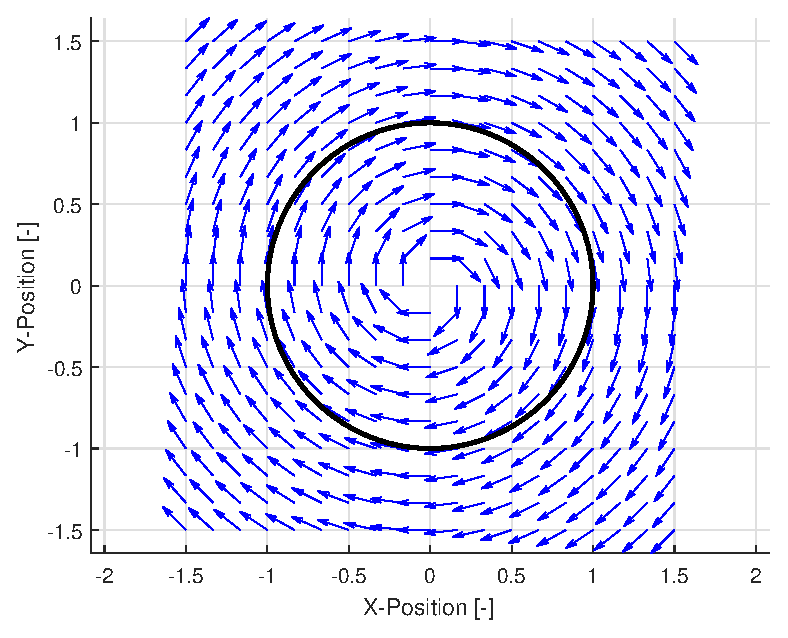
\includegraphics[width=0.7\linewidth]{Circ}
	\caption{GVF Circulation Field around Circle}
	\label{fig:circ}
\end{figure}
\begin{figure}[H]
	\centering
	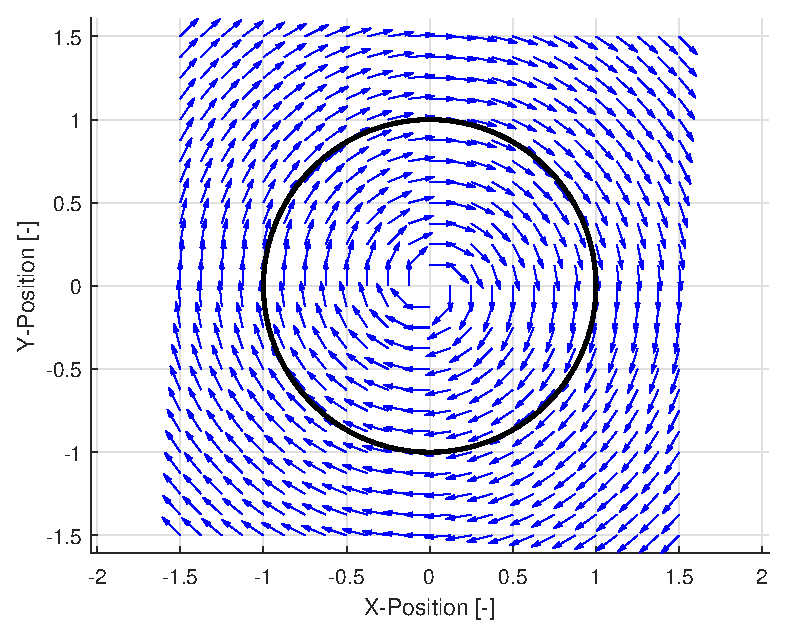
\includegraphics[width=0.7\linewidth]{Circnorm}
	\caption{GVF Circulation Field around Circle Normalized Vectors}
	\label{fig:circn}
\end{figure}
\begin{figure}[H]
	\centering
	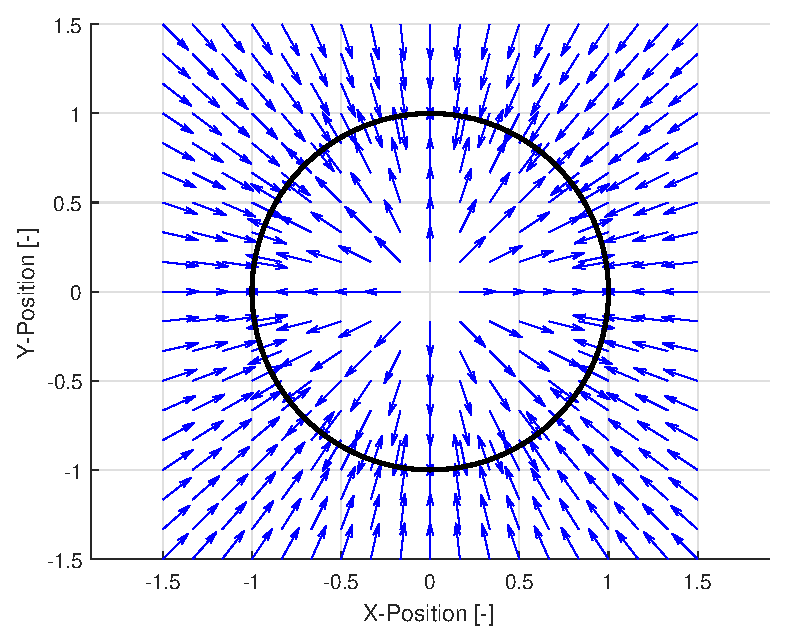
\includegraphics[width=0.7\linewidth]{Conv}
	\caption{GVF Convergence Field around Circle}
	\label{fig:Conv}
\end{figure}
\begin{figure}[H]
	\centering
	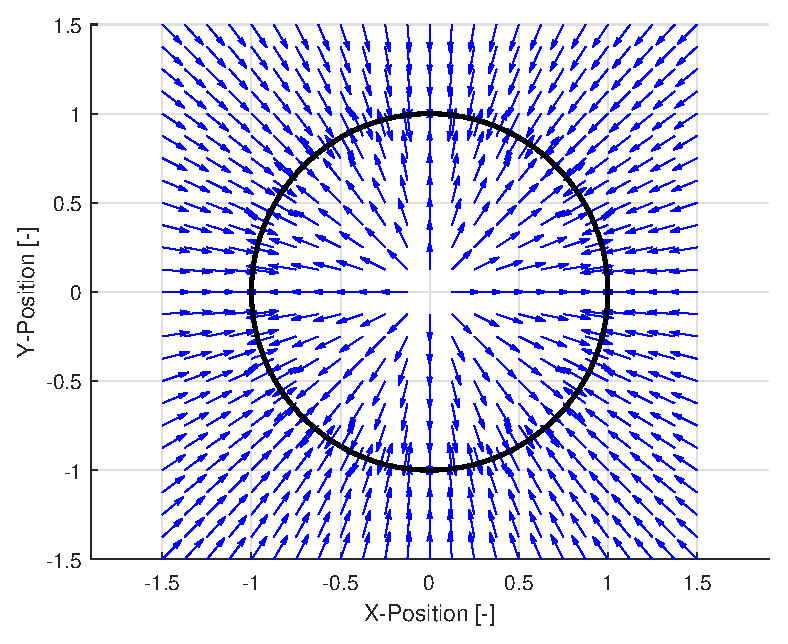
\includegraphics[width=0.7\linewidth]{Convnorm}
	\caption{GVF Convergence Field around Circle Normalized Vectors}
	\label{fig:Convn}
\end{figure}
\begin{figure}[H]
	\centering
	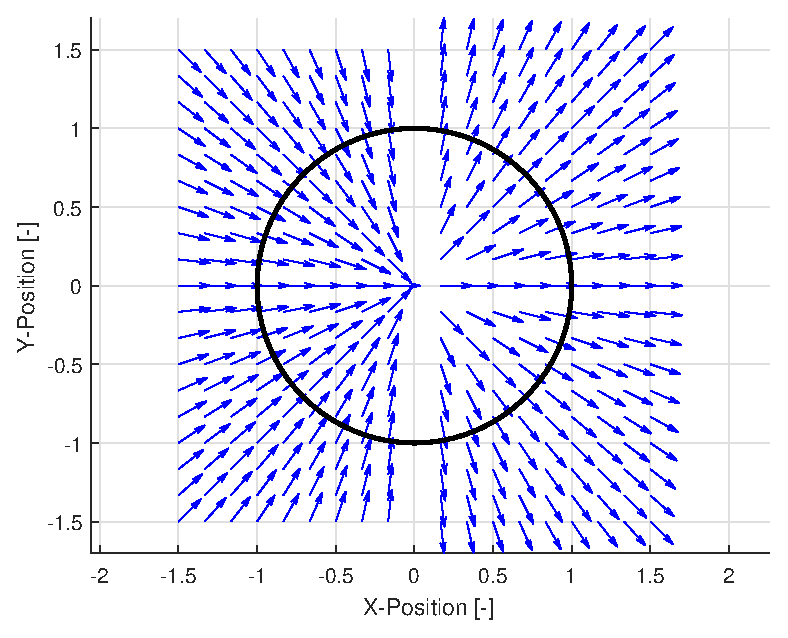
\includegraphics[width=0.7\linewidth]{TV}
	\caption{GVF Time Varying Field around Circle}
	\label{fig:TV}
\end{figure}
\begin{figure}[H]
	\centering
	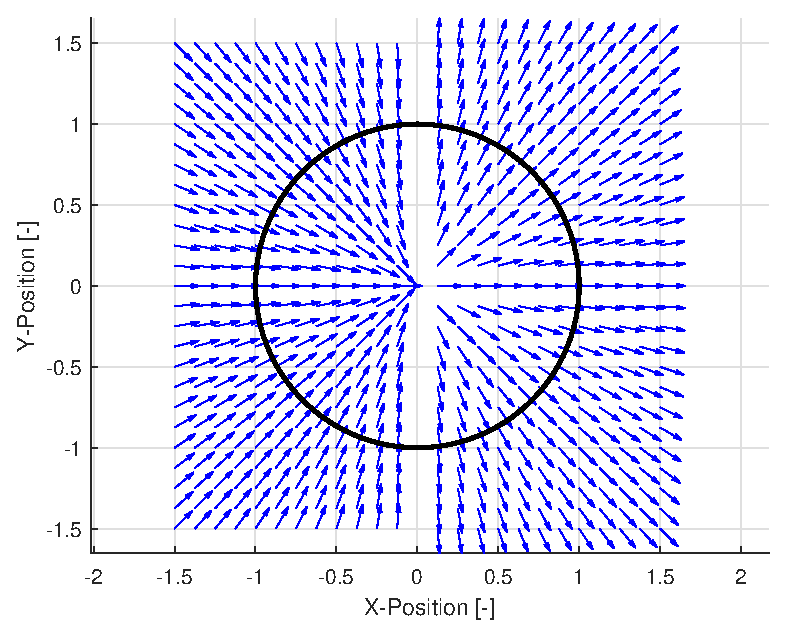
\includegraphics[width=0.7\linewidth]{TVnorm}
	\caption{GVF Time Varying Field around Circle Normalized Vectors}
	\label{fig:TVn}
\end{figure}
\begin{figure}[H]
	\centering
	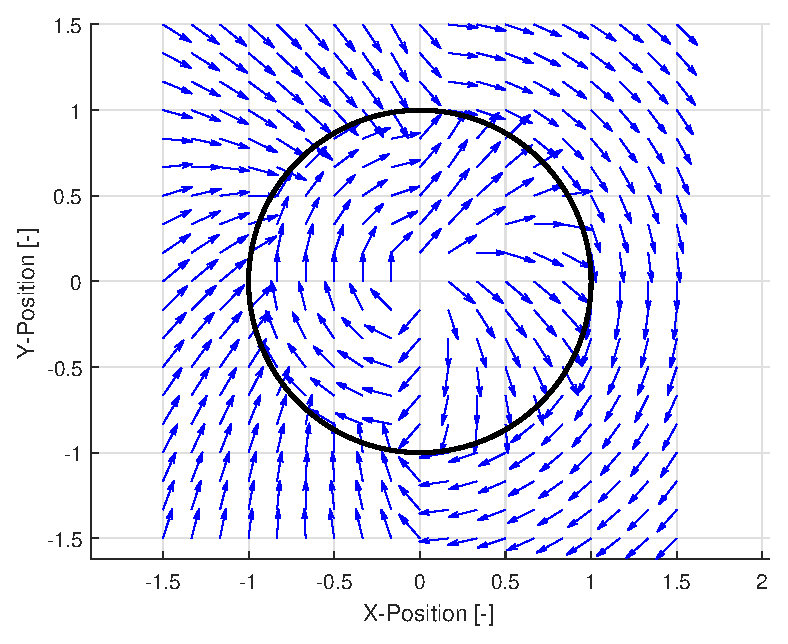
\includegraphics[width=0.7\linewidth]{All}
	\caption{Total Vector Field}
	\label{fig:all}
\end{figure}
\begin{figure}[H]
	\centering
	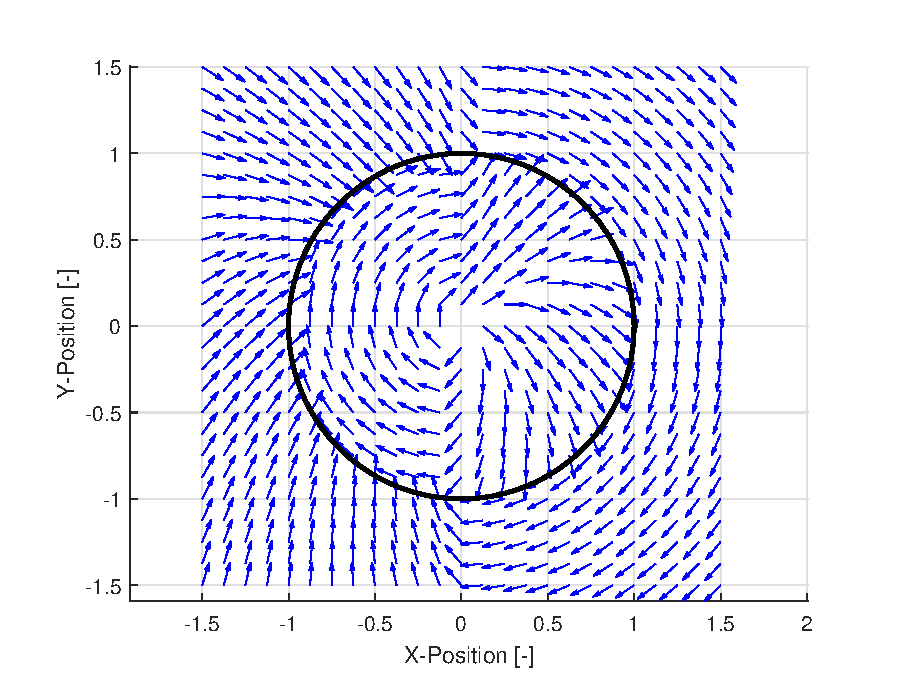
\includegraphics[width=0.7\linewidth]{Allnorm}
	\caption{Total Vector Field Normalized Vectors}
	\label{fig:alln1}
\end{figure}

\section{VF Guidance Performance}
Simulation of a Dubin's vehicle as previously described using the GVF and Lyapunov VF was performed to compare the found methods of circumnavigating a moving target. Three methods simulated were the GVF using summing and normalized vectors and then the Lyapunov circle vector field. All three of the vector fields provided enough guidance to the Dubin's vehicle using only the heading angle to circumnavigate a moving target. The differences in performance are the convergence time, circular tracking error, and stability. Simulations of a moving target that changes direction three times at a constant speed (1) with a circumnavigation radius of 1, a Dubin's vehicle at constant speed (5) and turn radius (20 deg/sec) with GVF parameters of (G=H=L=1) was performed. The VF component summing method (Equation \ref{eq:vfcomponent}) converges upon the circle the quickest and has the smallest tracking error, but contains twitching or chattering while following the circle. The VF normalization (Equation \ref{eq:vfcomponentmod}) has similar convergence time to the summing and does not track as well, but has a much larger oscillation error from the circle without any twitching. Finally, the Lyapunov VF provided the slowest response and highest tracking error with about the same oscillation or deviation from the circle while tracking. 
\begin{figure}[H]
	\centering
	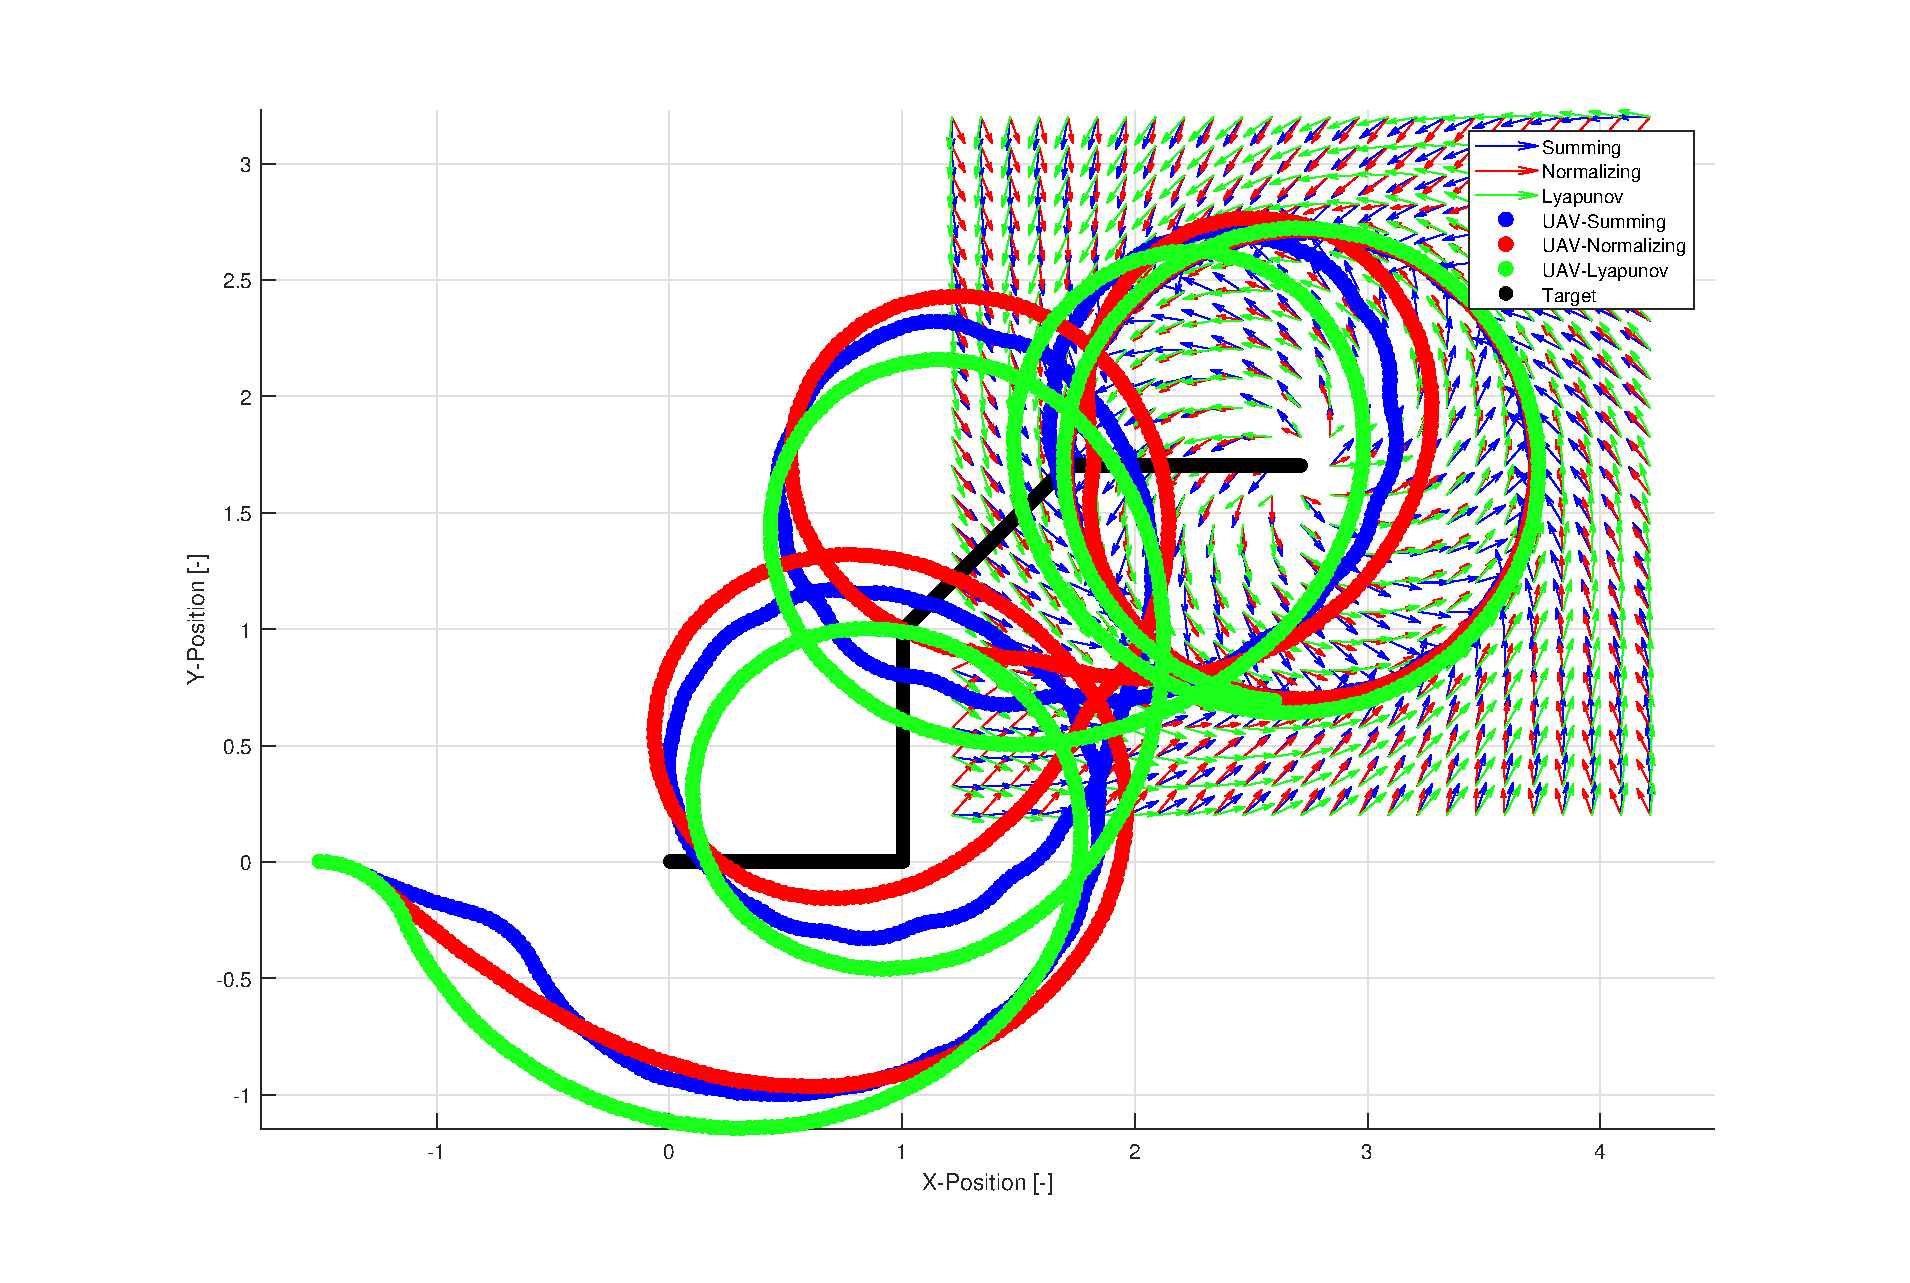
\includegraphics[width=6.5in]{moving3uavresult.eps}
	\caption{Total Vector Field Normalized}
	\label{fig:alln2}
\end{figure}
The steady state tracking error once the target has stopped moving shows a tracking error of high twitching with the summing, smooth constant small error with the GVF normalization, and higher error with the Lyapunov VF. The tracking performance error, defined as the distance from the circulation or radius point of the moving target, is shown in Figure \ref{fig:move_error}. Overall, the UAV controller would need to decide between (or switch) the smooth guidance of normalization or the tracking performance of the summing GVF. 

\begin{figure}[H]
	\centering
	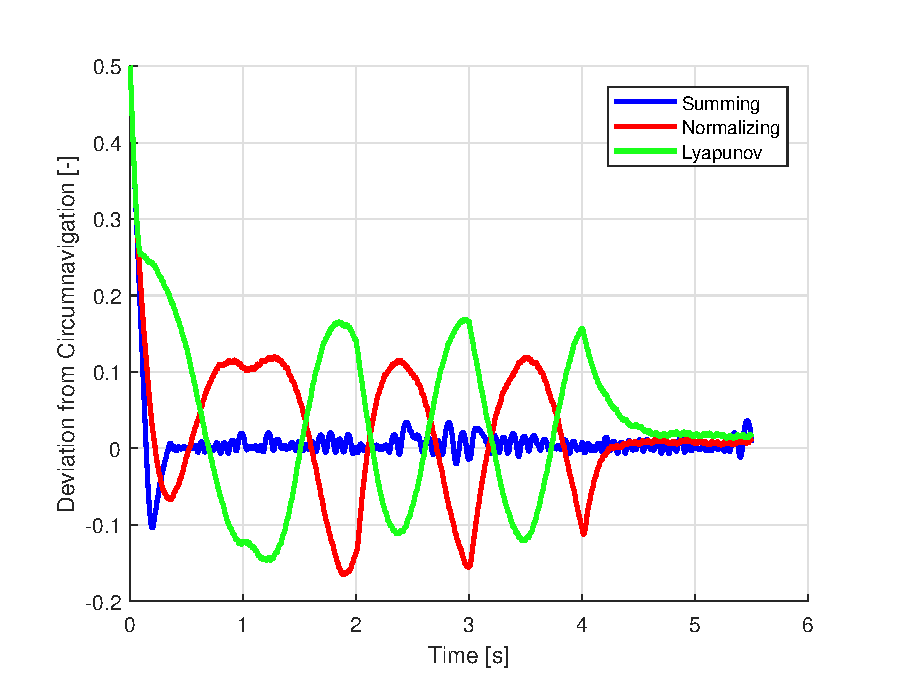
\includegraphics[width=0.7\linewidth]{moving3uaverror.eps}
	\caption{Total Vector Field Normalized}
	\label{fig:move_error}
\end{figure}

\subsection{Obstacle Avoidance}
Obstacle avoidance can be achieved by using only the inverted convergence vector with an activation function. The inverted convergence, with a minimal radius circle, will always push away from the center point. The radius must be much smaller than the actual obstacle because the field direction reverses once the radius threshold has been crossed. An activation function was used to express the radius of the obstacle and to reduce the avoidance contribution of a circular obstacle of radius, $R$, as the distance from the center, $d$, decreases (Equation \ref{eq:tanh} and is show in Figure \ref{fig:2avoid}). The final convergence vector (Equation \ref{eq:vftotal}) is combined with the 'G' factor to add additional vectoring magnitude, the activation function, and typical convergence vector calculation as before. The GVF does not account for distance from the path to increase or decrease aspects of guidance, although Gon\c{c}alves did propose varying G and H proportionally to distance and performance parameters to emphasize parts of the GVF as an object moves through the field. Placement of the obstacle is performed by selection an $x$ and $y$ coordinate and a radius. The vector calculated from the obstacle is added to the guidance vector and any other obstacle vectors to produce a final guidance vector. No guarantee is provided that the UAV will not violate the obstacle's radius, but several simulations have shows that a UAV on direct course for the obstacle was successfully diverted as shown in Figure \ref{fig:2avoid}. The simulated UAV was following a moving target at a radius of 1, internal obstacle radius of (0.01), P radius of 1, a 2:1 velocity ratio, G=H=L=1 and managed to avoid each obstacle.


\begin{equation} \label{eq:tanh}
P = R\frac{\tanh \left( 2 \pi d - \pi \right)+1}{2}
\end{equation}

\begin{equation} \label{eq:vfavoid}
\overrightarrow{A} = -G  \lVert \overrightarrow{V}_{conv} \rVert P
\end{equation}
\begin{equation} \label{eq:vftotal}
\overrightarrow{V}_{total} = \overrightarrow{V} + \sum_{i=1}^{n-1} \overrightarrow{A}_i
\end{equation}
\begin{figure}[H]
	\centering
	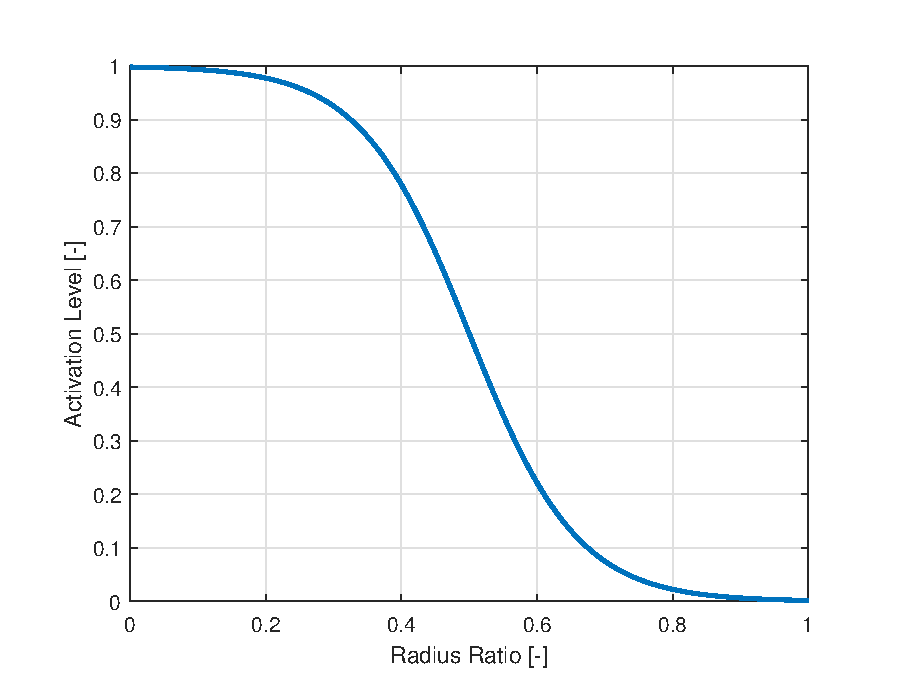
\includegraphics[width=0.7\linewidth]{tanh}
	\caption{Activation Function}
	\label{fig:tanh}
\end{figure}

\begin{figure}[H]
	\centering
	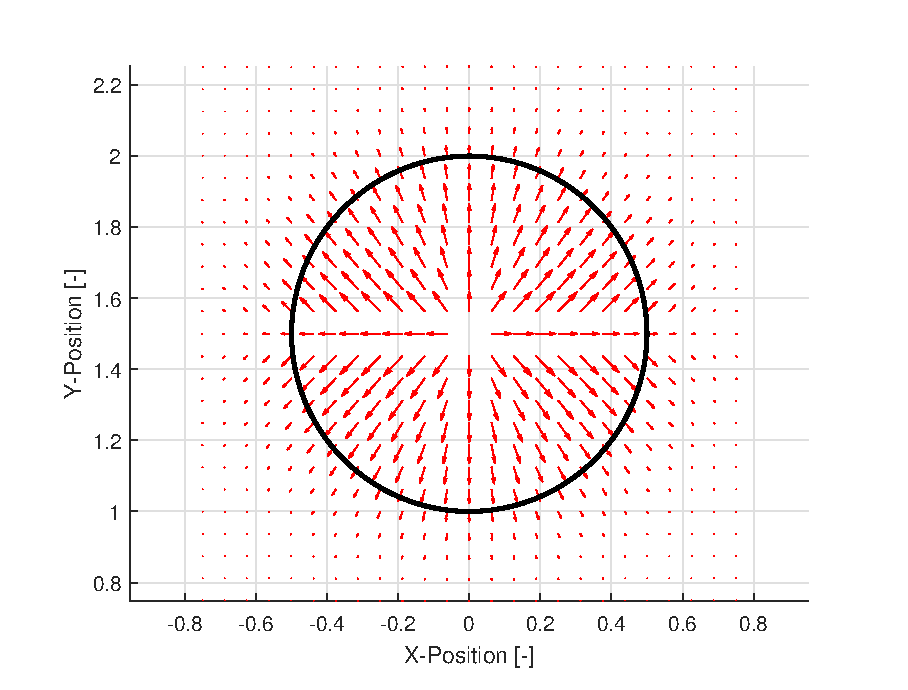
\includegraphics[width=0.7\linewidth]{avoid}
	\caption{Obstacle Vector Field Example}
	\label{fig:avoid}
\end{figure}
\begin{figure}[H]
	\centering
	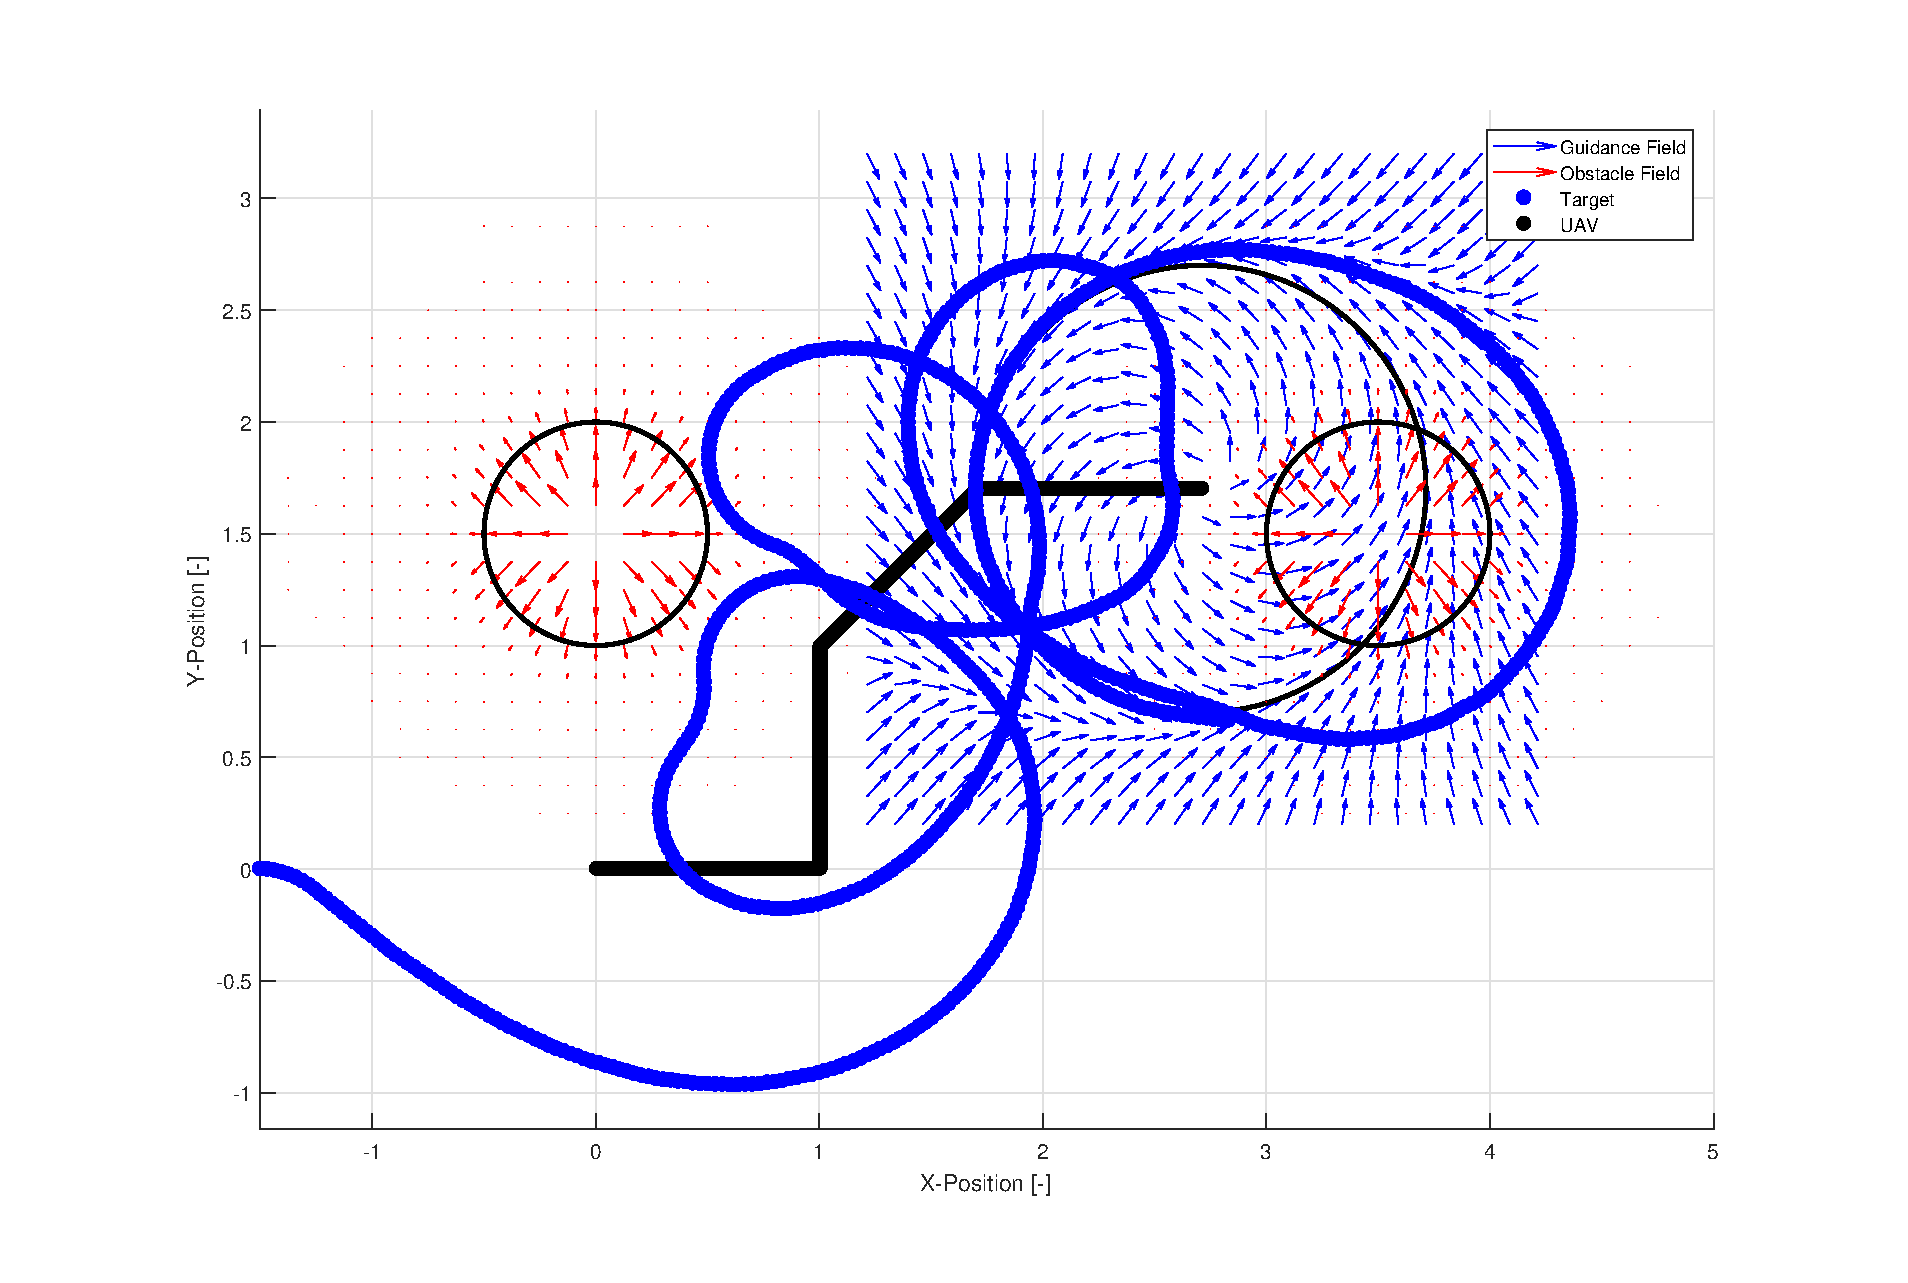
\includegraphics[width=6.5in]{avoid_color_legend}
	\caption{Obstacle Vector Field UAV Example}
	\label{fig:2avoid}
\end{figure}

\section{Conclusion}

Vector field guidance of a UAV has several benefits over traditional guidance law methods. The advantages include simplicity of calculations, no time history required, and finally the ability to include obstacle avoidance. Research was performed into which type of VF to use for UAV guidance, parameters of the VF, and an obstacle avoidance method was developed. The target following performance of circumnavigation was tested using a Dubins path follower with outstanding performance. Obstacle avoidance was included by utilizing an inverse convergence field with an activation function to drive away vehicles. The investigated VF guidance for loitering or circumnavigation a moving target and avoiding obstacles that may exist on the ground or air was successfully achieved in simulation.

\bibliography{VF}

\end{document}
